
\begin{figure}
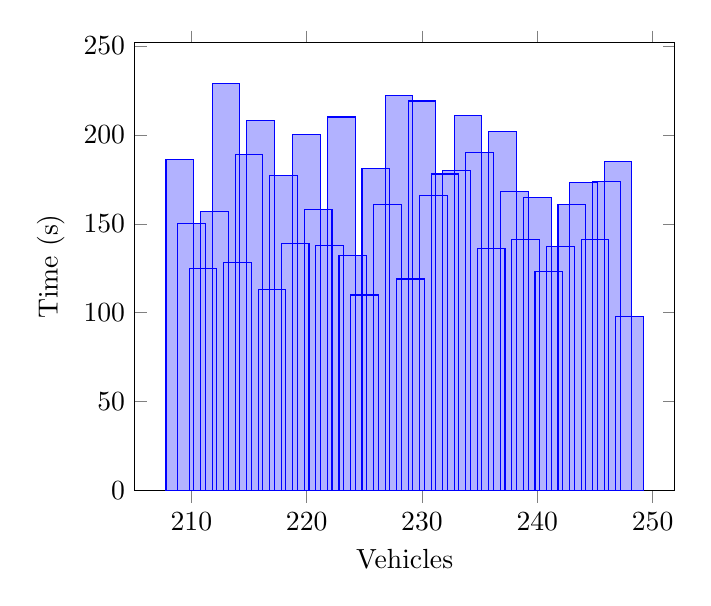
\begin{tikzpicture}
\begin{axis}[
legend style={anchor=west},
xlabel=Vehicles,
ylabel=Time (s),
ymin=0,
ybar,
]
\addplot coordinates {
(248, 98)
(238, 168)
(239, 141)
(234, 211)
(235, 190)
(236, 136)
(237, 202)
(231, 166)
(232, 178)
(233, 180)
(230, 219)
(228, 222)
(245, 141)
(244, 173)
(247, 185)
(246, 174)
(241, 123)
(240, 165)
(243, 161)
(242, 137)
(221, 158)
(215, 189)
(222, 138)
(218, 177)
(219, 139)
(209, 186)
(216, 208)
(217, 113)
(214, 128)
(212, 157)
(213, 229)
(210, 150)
(211, 125)
(229, 119)
(227, 161)
(226, 181)
(225, 110)
(224, 132)
(223, 210)
(220, 200)
};

\end{axis}
\end{tikzpicture}
\label{tik:time:0:97}
\caption{0 percent diving with GSC on route $97$}
\end{figure}
